%\graphicspath{{../images/}}
\section{Обзор методов шумоподавления}
\subsection{Постановка задачи}
Будем считать, что существует исходное изображение $x$, которое не искаженно шумом. После процедуры наложения шума $n$, получаем шумное изображение $y$. Степень зашумленности изображения можно описать с помощью отношения сигнал/шум.
 Отношение сигнал/шум (SNR) - безразмерная величина, равная отношению мощности сигнала на мощность шума. В текущих обозначениях получим:
\begin{equation}
	SNR = \frac{P_y}{P_n}
\end{equation} 
где
\begin{itemize}
	\item $P_y$ - мощность сигнала (изображения)
	\item $P_n$ - мощность шума
\end{itemize}

Значит, чтобы уменьшить влияния шума на изображения, необходимо либо увеличить мощность сигнала, либо уменьшить количество шума. Вторым методом и занимаются алгоритмы шумоподавления.
В данной ВКР будем считать, что изображение $x$ будет искаженно аддитивным шумом $n$ и не зависит от исходного изображения. Искаженное изображение будет обозначаться $y$. Опишем это следующим образом.
\begin{equation}
	y = x + n
\end{equation}
Целью шумоподавления является нахождение исходного изображения $x$, при этом слагаемое $n$ неизвестно, а доступно лишь только зашумленное изображение $y$. В реальной жизни невозможно достоверно точно восстановить изображение $x$.



\subsection{Модели шума}
Шум изображения - это случайное изменение яркости или цветовой информации на изображениях и, как правило, аспект электронного шума. Шум может как зависеть от изображения так и быть независимым. Является нежелательным побочным продуктом захвата изображения, который скрывает желаемую информацию.
лао
Шум изображения может варьироваться от практически незаметных пятен на цифровой фотографии, сделанной при хорошем освещении, до оптических и радиоастрономических изображений, которые почти полностью представляют собой шум, из которого небольшое количество информации может быть получено с помощью сложной обработки. Такой уровень шума был бы недопустим на фотографии, так как было бы невозможно даже определить объект\cite{Noise}.

Характер проблемы удаления шума зависит от типа шума, повреждающего изображение\cite{Gonzalez}: 
\begin{itemize}
	\item гауссовский шум
	\item пуассоновский шум
	\item шум Релея
	\item шум Эрланга
	\item импульсный шум
	\item равномерный шум
	\item экспоненциальный шум;
\end{itemize}

Ниже будут подробно рассмотрены одни из самых популярных моделей шума.
\subsubsection{Гауссовский  шум}
Модель гауссовского шума является одной из самых популярных моделей шума в задачах шумоподавления, так как он описывает естественные причины появления шумах, так же это обусловленно математической простотой описания данного типа шума.
Гауссовский шум - это модель теплового шума, который в свою очередь вызван беспорядочным движением зарядов в полупроводнике из-за теплового хаотического движения носителей заряда\cite{Polupro}.
Гауссовский шум является аддитивным, поэтому процесс искажения цифрового изображения можно описать следующей формулой:
\begin{equation}
	y = x + n
\end{equation}
где
\begin{itemize}
	\item y - зашумленное изображение 
	\item x - исходное изображение
	\item n - случайная величина имеющая гауссовское распределение.
\end{itemize}
Гауссовский шум можно описать плотностью вероятности имеющий вид\cite{gauss}:
\begin{equation}
	P(z)=\frac{1}{\sigma\sqrt{2\pi}}e^{\frac{(z-\mu)^2}{2\sigma^2}}
\end{equation}
где
\begin{itemize}
	\item $P(z)$ - функция плотности распределения вероятностей гауссовской случайной величины
	\item $z$ - значение яркости
	\item $\sigma$ - среднеквадратичное отклонение
	\item $\mu$ - среднее значение
\end{itemize}
Как правило при моделировании шума на изображение, параметр $\mu$ берётся равным 0.

\subsubsection{Пуассоновский шум}
Немаловажным на практике является также пуассоновский шум, известный так же как фотонный шум. Он является зависимым от интенсивности потока фотонов в окрестности исследуемого пикселя.
Датчики изображения измеряют освещенность сцены путем подсчета количества дискретных фотонов, падающих на датчик в течение заданного интервала времени. В полупроводниковых датчиках фотоэффект используется для преобразования фотонов в электрон. Независимость случайных индивидуальных приходов фотонов приводит к фотонному шуму, зависящей от сигнала форме неопределенности, которая является свойством самого базового сигнала\cite{poisson}.
Количество фотонов, которые буду задетектированы описываются пуассоновским распределением.

Распишем выражения дискретного распределения вероятностей:
\begin{equation}
	P(X=k)=\frac{N^k}{k!}e^{-N}
\end{equation}
где:
\begin{itemize}
	\item $P(X=k)$ - вероятность того, полученная интенсивность примет значение равное k
	\item $X$ - интенсивность
	\item $k$ - интенсивность, которая может быть получена
	\item $N$ - истинная интенсивность
\end{itemize}

Зависимость шума, от сигнала, в случае пуассоновского распределения можно описать с помощью SNR\cite{Kumar}:
\begin{equation}
	SNR=\frac{N}{\sqrt{N}}
\end{equation}
где $N$ мощность сигнала. Можно видеть, что с увеличением мощности сигнала, так же увеличивается мощность шума. Но при этом скорость возрастания мощности сигнала больше, чем скорость возрастания мощности шума. Это значит, что если в качестве сигнала мы возьмем изображение, то влияние пуассоновского шума на него будет отчетливее видно при низкой интенсивности исходного изображения.
\subsection{Простейшие алгоритмы шумоподавления}
\subsubsection{Демонстрация работы алгоритмов шумоподавления}
\paragraph{Изображение без шума}
Для демонстрации работы фильтров будет использовано следующее изображение.
\begin{figure}[H]
	\center{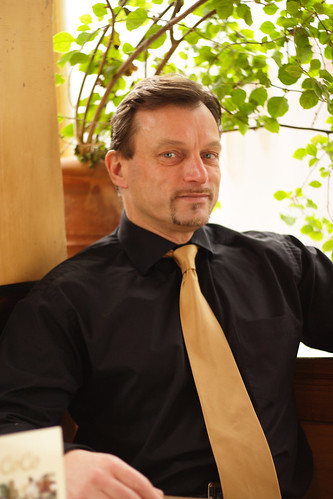
\includegraphics[scale=0.5]{orig}}
	\caption{Изображение взятое из открытой базы данных \cite{imageNet}}
	\label{img:orig}
\end{figure}
\paragraph{Схема процесса добавления шума}
Ниже приведена схема алгоритма добавления гауссовского шума с дисперсией $\sigma^2$ и подробное её описание:
\begin{figure}[H]
	\center{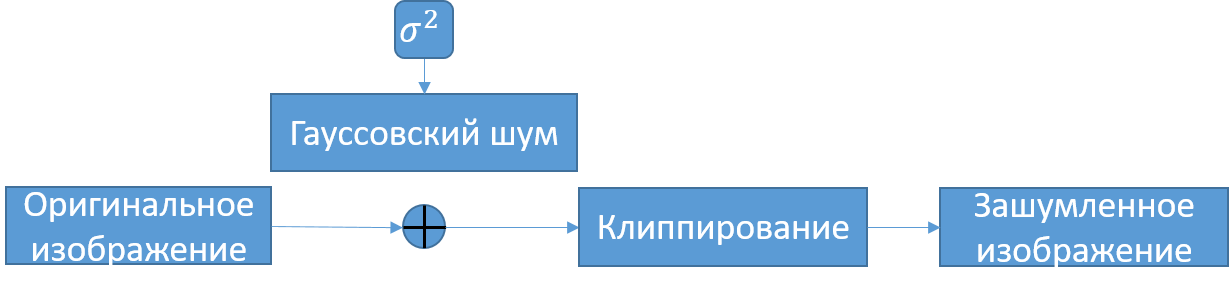
\includegraphics[scale=0.7]{circuitAddNoise}}
	\caption{Схема алгоритма добавления шума}
\end{figure}

На вход поступают изображение,  на которое необходимо наложить шум и значение дисперсии. При это значения интенсивности изображения  должны находится в промежутке $[0,1]$. Генерируется матрица имеющая размер такой же как и у входного изображения, элементы матрицы имеют гауссовское распределение с дисперсией равной $\sigma^2$, и средним значением равным 0. Затем гауссовский шум складывается с изображением. Полученная сумма клиппируется, после этого минимальное значение данной суммы равно 0, а максимальное 1.
\paragraph{Критерий оценки алгоритмов шумоподавления}
В качестве критерия оценки алгоритмов будет использовано пиковое соотношение сигнал/гум (PSNR). PSNR подробно будет разобрано в \ref{sec:PSNR}. Пока лишь будет представлена формула и её описание:
\begin{equation}
PSNR = 10log_{10}(\frac{MAX_I^2}{MSE})
\end{equation}
где 
\begin{itemize}
	\item $MAX_I$ - максимально возможное значения пикселя
	\item $MSE = \frac{1}{nm}\sum_{i=0}^{n}\sum_{j=0}^{m}(x_{i,j} - y_{i,j})^2$ - средний квадрат ошибки между оригинальным изображением x и искаженным y.
	\item m,n - высота и ширина изображения
\end{itemize}
\paragraph{Зашумленное изображение}
В качестве примеру на изображение рис. \ref{img:orig} будет накладываться гауссовский шум  с дисперсией равной  0.05.
\begin{figure}[H]\label{img:noised}
	\center{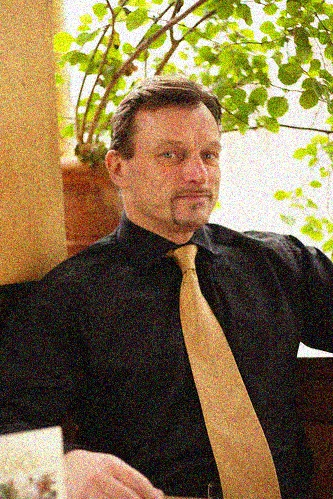
\includegraphics[scale=0.5]{noised}}
	\caption{Изображения с добавлением аддитивного гауссовского шума с $\sigma^2=0.05$}
\end{figure}
Для зашумленного изображения PSNR$=23.46$.
\subsubsection{Фильтр скользящего среднего}
Первые фильтры были линейными, они были основаны на идее, что пиксели в некоторой малой окрестности имеют примерно одинаковые значения интенсивности. Поэтому если представлять каждый пиксель в виде суммы пикселей в окрестности, то это поможет избавиться от шума. Такой фильтр называется фильтр скользящего среднего. Фильтр скользящего среднего задается квадратной матрицей с радиусом r, где каждый элемент матрицы равен $\frac{1}{r^2}$.
\begin{figure}[H]
	\center{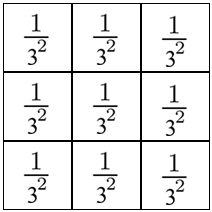
\includegraphics[scale=0.5]{kernelBox}}
	\label{img:kernelBox}
	\caption{Пример ядра фильтра скользящего среднего размером $3\times 3$}
\end{figure}
Ниже представлен пример работы фильтра. В данном случае $PSNR=20.16$.
\begin{figure}[H]
	\center{
\includegraphics[scale=0.5]{box11}}
	\caption{Результат применения фильтра скользящего среднего размером $11\times 11$}
\end{figure}
\begin{figure}[H]
	\center{
\includegraphics[trim={5cm 10cm 10cm 5cm},scale=3, clip]{box11}}
	\caption{Артефакты при применении фильтра скользящего среднего размером $11\times 11$}
\end{figure}
Как можно видеть, результат работы  фильтра скользящего среднего имеет артефакты в виде горизонтальных и вертикальных линий. Это является причиной почему данный фильтр не используют на практике.
\subsubsection{Фильтр Гаусса}
Улучшением идеи  фильтра скользящего среднего стал гауссов фильтр. В отличии от ядра  фильтра скользящего среднего фильтра, значения ядра фильтра Гаусса вычисляются с помощью функции Гаусса от двух переменных :

\begin{equation}
	G(x,y) = \frac{1}{\sqrt{2\pi}\sigma^2}e^{\frac{x^2+y^2}{2\sigma^2}}
\end{equation}
где
\begin{itemize}
	\item $x,y$ - координаты ядра
	\item $\sigma$ среднеквадратичное отклонение
\end{itemize}

Параметр $\sigma$ обозначает насколько сильно будет размыто изображение, соотвественно от $\sigma$ зависит и радиус ядра фильтра. Т.е. $r=3\sigma$, соотвественно чем больше сигма, тем больше размытие изображения. Ниже представлены графики одномерное функции Гаусса с различными значениями $\sigma$.

\begin{figure}[H]
	\center{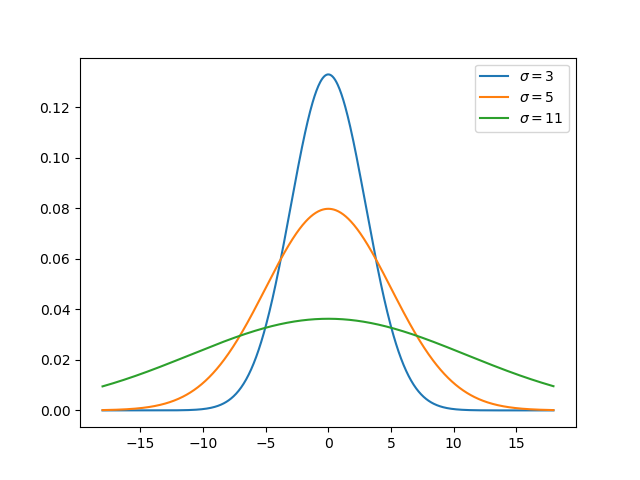
\includegraphics[scale=0.9]{plotGauss.png}}
	\caption{Графики функции Гаусса с параметром $\sigma = 3,5,11$}
\end{figure}

Применим фильтр Гаусса для рис. \ref{img:orig} с различными параметрами $\sigma$.

\begin{figure}[H]
	\centering
	\subfigure[]{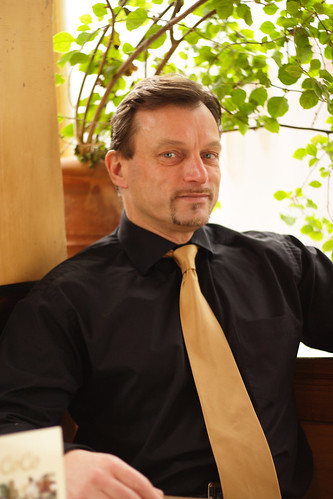
\includegraphics[scale=0.45]{orig}
		\label{img:orig1}
	}
	\hspace{0.0125ex}
	\subfigure[]{
\includegraphics[scale=0.45]{gauss3.png}
		\label{img:gauss3}
	}
	\hspace{0.0125ex}
	\subfigure[]{
\includegraphics[scale=0.45]{gauss11.png}
		\label{img:gauss11}
	}
	\caption{Пример работы гауссовского фильтра: \subref{img:orig1} оригинал; \subref{img:gauss3} с радиусом 3; \subref{img:gauss11} с радиусом 11}
\end{figure}
Для рис. \ref{img:gauss3} PSNR$=21.96$, а для \ref{img:gauss11} PSNR$=17.18$.
\paragraph{Достоинства и недостатки  фильтра скользящего среднего и фильтра Гаусса}
Преимуществом первых фильтров является простая реализация и быстрая скорость работы. Так как процесс шумоподавления, можно представить в виде поэлементного умножения спектрального образа шума на спектральный образ изображения. Но они также обладают одним существенным недостатком. Данные фильтры размывают края, это может негативно сказываться на алгоритмах компьютерного зрения.
\subsubsection{Медианный фильтр}
Избавиться от указанного выше недостатка попытался медианный фильтр. Он основан на той идее, что пиксели в некоторой малой окрестности имеют приблизительно равную интенсивность, а шум, соотвественно сильно отличается. Поэтому для пикселя, для которого вычисляется новое значения, берутся пиксели в некоторой окрестности. Как правило, это квадрат с радиусом r. Данные пиксели сортируются по возрастанию или убыванию и новым значением объявляется то, что находится в середине.

Продемонстрируем на примере работу фильтра.

\begin{figure}[H]
		\centering
	\subfigure[]{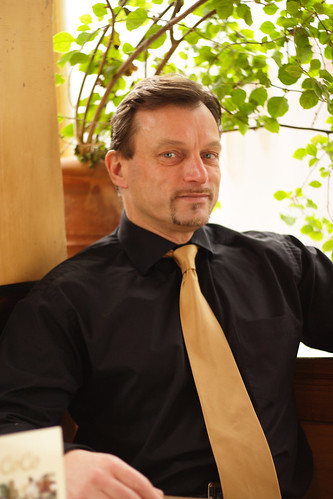
\includegraphics[scale=0.45]{orig}
		\label{img:orig2}
	}
	\hspace{0.0125ex}
\subfigure[]{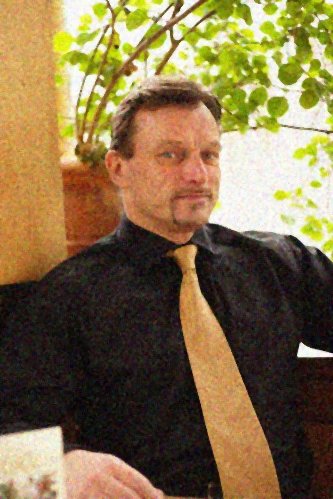
\includegraphics[scale=0.45]{median3.png}
		\label{img:median3}
	}
\hspace{4ex}
\subfigure[]{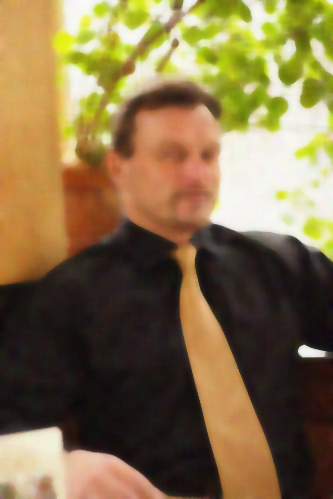
\includegraphics[scale=0.45]{median11.png}
	\label{img:median11}
}
	\caption{Результат работы медианного фильтра:\subref{img:orig2} оригинал} ; \subref{img:median11} с радиусом 11;\subref{img:median3} с радиусом 3;
\end{figure}
Для рис. \ref{img:median3} PSNR$=26.83$, а для \ref{img:median11} PSNR$=21.45$.
\paragraph{Достоинства и недостатки медианного фильтра}
Данный алгоритм работает хорошо, только с импульсным шумом, что сильно ограничивает его область использования. Но главным недостатком фильтра является то, что изображение теряет своё визуальное качество.
\subsection{Проблемы распознавания лиц при добавлении шума}
Как утверждалось выше, наличие шума на изображении снижает эффективность работы некоторых методов обработки изображений. Продемонстрируем это на примере одного из самых распространенных алгоритмов компьютерного зрения - распознавание лиц.
Воспользуемся электронным ресурсом \cite{FaceDetections}, который позволяет обнаруживать лица. В качестве тестовых данных возьмем изображение из открытой базы данных ImageNet \cite{imageNet}.
\begin{figure}[H]
	\center{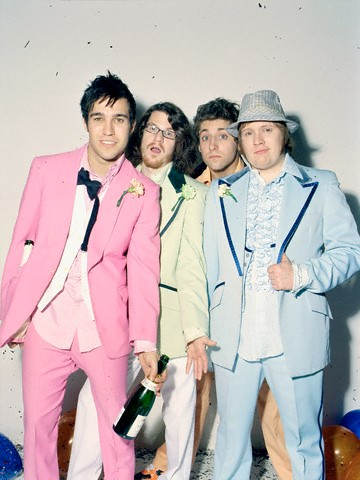
\includegraphics[scale=0.65]{faceOrig}}
	\caption{Фотография четырёх людей без добавления  шума}
\end{figure}
Результатом работы алгоритма является загруженное изображение, на котором зеленным цветом выделены найденные лица, так же на изображении обозначенны красным цветом некоторые черты лица: рот, глаза, нос и брови.
\begin{figure}[H]
	\center{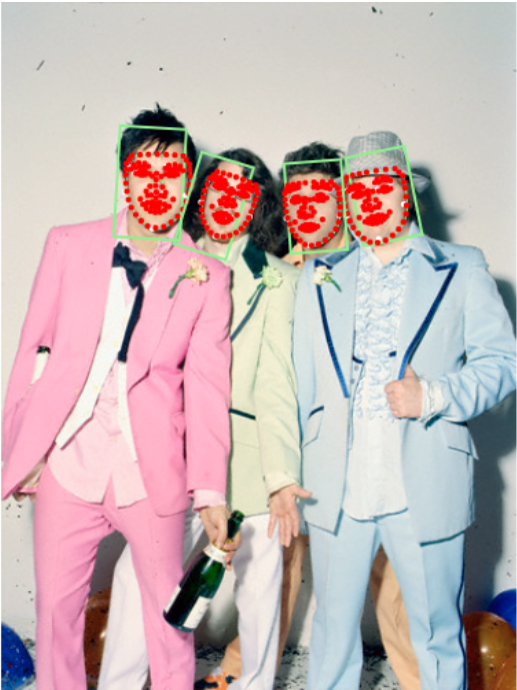
\includegraphics[scale=0.65]{faceOrigRes}}
	\caption{Результат работы распознавания лиц изображения не искаженного шумом}
\end{figure}
Посмотрим, как повлияет добавление шума, на эффективность работы алгоритма. Для это добавим аддитивный гауссовский шум сразличной дисперсией $\sigma^2=0.01, 0.05, 0.15$. 
\begin{figure}[H]
	\begin{minipage}[H]{0.32\linewidth}
		\center{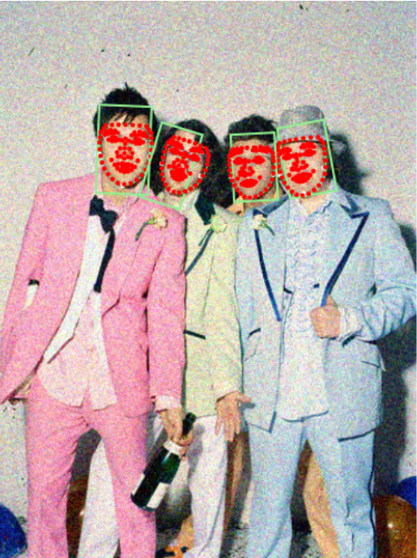
\includegraphics[scale=0.8]{faceNoise1} \\ а) $\sigma^2=0.01$}
	\end{minipage}
	\begin{minipage}[H]{0.32\linewidth}
		\center{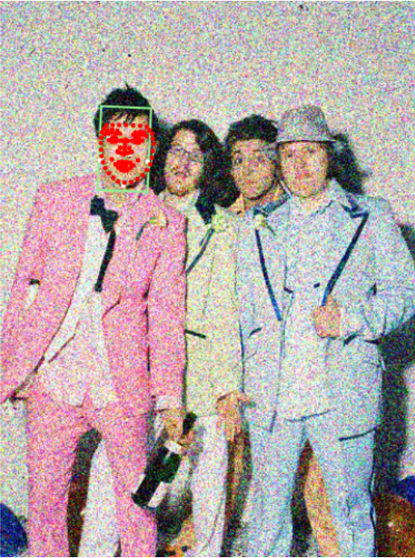
\includegraphics[scale=0.8]{faceNoise5} \\ б) $\sigma^2=0.05$}
	\end{minipage}
	\begin{minipage}[H]{0.32\linewidth}
		\center{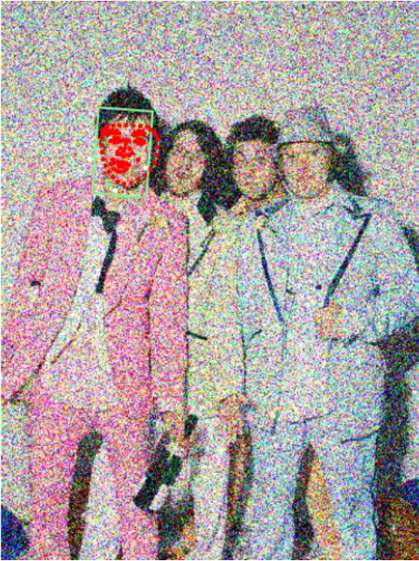
\includegraphics[scale=0.8]{faceNoise15} \\ в) $\sigma^2=0.15$}
	\end{minipage}
	\caption{Распознавание лиц на изображениях с шумом}
\end{figure}
Как можно видеть, только на изображении с $\sigma^2=0.01$ количество лиц осталось прежним, для остальных же удалось распознать только одно лицо.

Попробуем применить гауссовский фильтр с размером ядра равным 3.
\begin{figure}[H]
	\begin{minipage}[H]{0.32\linewidth}
		\center{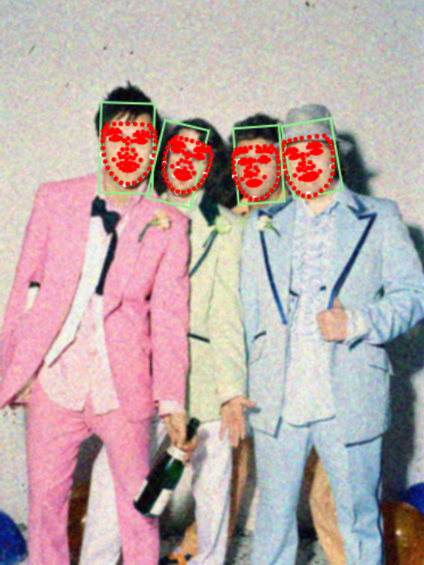
\includegraphics[scale=0.8]{faceNoise31} \\ а) $\sigma^2=0.01$}
	\end{minipage}
	\begin{minipage}[H]{0.32\linewidth}
		\center{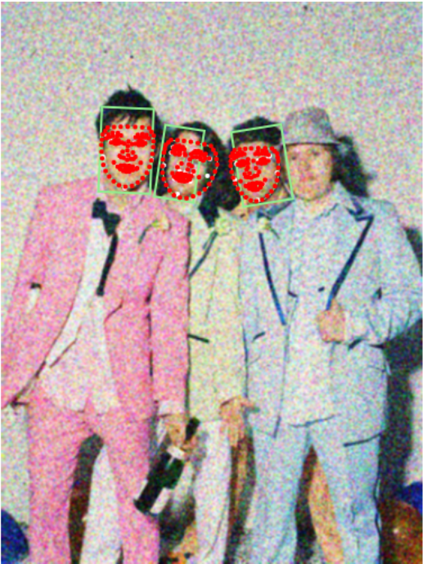
\includegraphics[scale=0.8]{faceNoise35} \\ б) $\sigma^2=0.05$}
	\end{minipage}
	\begin{minipage}[H]{0.32\linewidth}
		\center{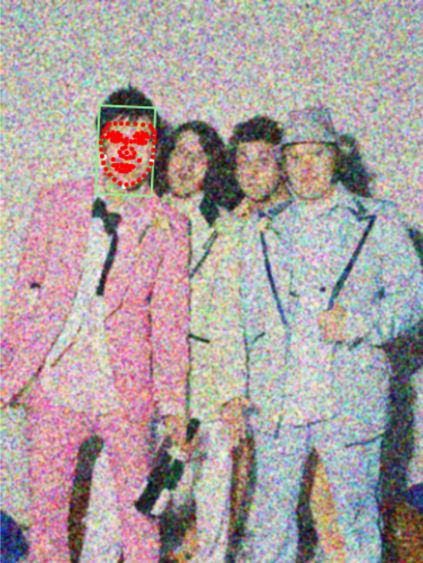
\includegraphics[scale=0.8]{faceNoise315} \\ в) $\sigma^2=0.15$}
	\end{minipage}
	\caption{Распознавание лиц на изображениях после применения гауссовского фильтра с радиусом 3}
\end{figure}
На изображения с $\sigma^2=0.01$ ничего не поменялось, но для фото с $\sigma^2=0.05$ результаты работы алгоритма улучшились. А именно удалось распознать уже 3 лица. Но на изображении с $\sigma^2=0.15$ всё так же удалось определить только одно лицо.

Увеличим радиус ядра до 5.
\begin{figure}[H]
	\begin{minipage}[H]{0.32\linewidth}
		\center{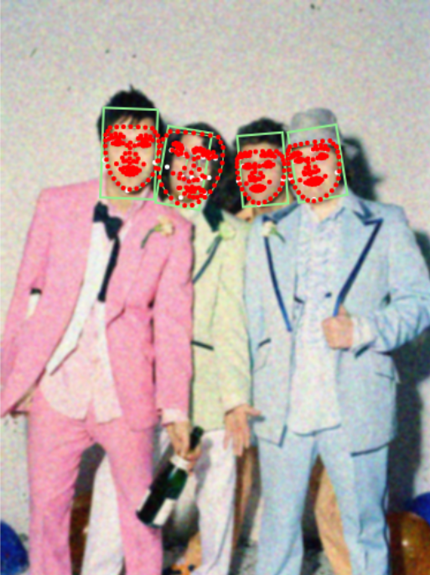
\includegraphics[scale=0.8]{faceNoise51} \\ а) $\sigma^2=0.01$}
	\end{minipage}
	\begin{minipage}[H]{0.32\linewidth}
		\center{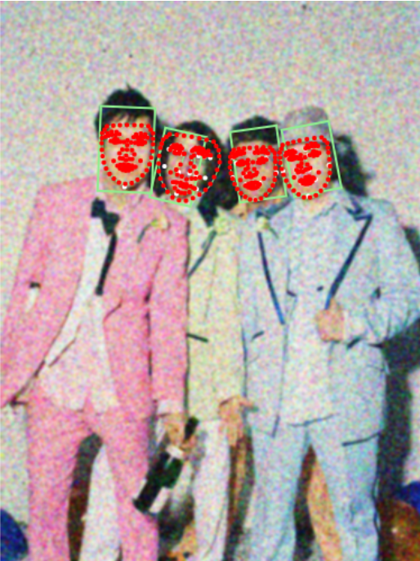
\includegraphics[scale=0.8]{faceNoise55} \\ б) $\sigma^2=0.05$}
	\end{minipage}
	\begin{minipage}[H]{0.32\linewidth}
		\center{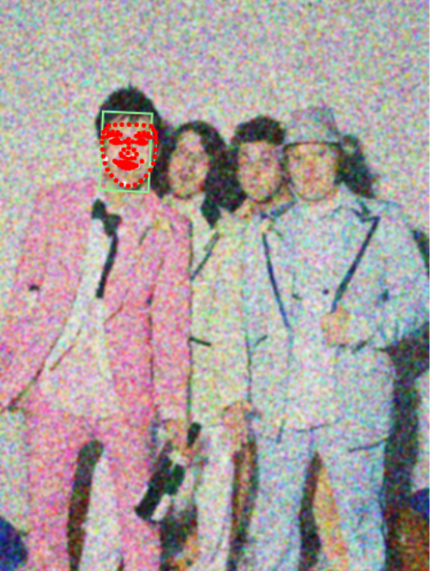
\includegraphics[scale=0.8]{faceNoise515} \\ в) $\sigma^2=0.15$}
	\end{minipage}
	\caption{Распознавание лиц на изображениях после применения гауссовского фильтра с радиусом 5}
\end{figure}
Благодаря увеличению размера ядра, удалось распознать 4 лица, на изображении с $\sigma^2=0.05$. Для фото с $\sigma^2=0.15$ ничего не изменилось. Однако для изображения с  $\sigma^2=0.01$ качество распознавания несколько ухудшилось, черты лица второго человека справа немного расплылись.
Возьмем ядро с радиусом 21.
\begin{figure}[H]
	\begin{minipage}[H]{0.32\linewidth}
		\center{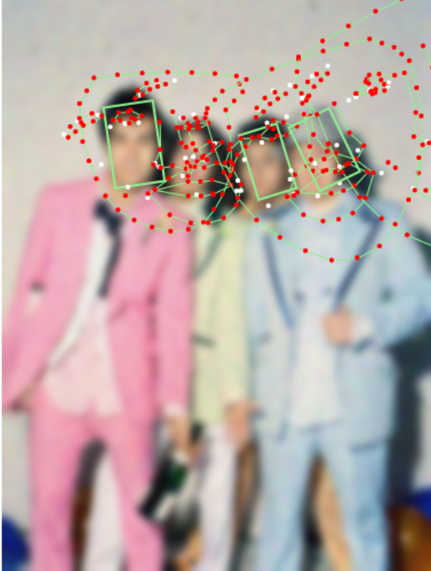
\includegraphics[scale=0.8]{faceNoise211} \\ а) $\sigma^2=0.01$}
	\end{minipage}
	\begin{minipage}[H]{0.32\linewidth}
		\center{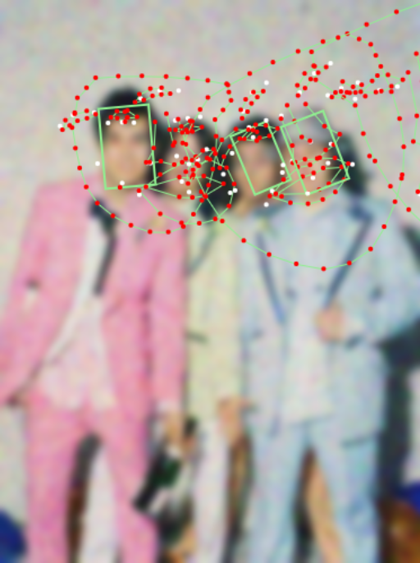
\includegraphics[scale=0.8]{faceNoise215} \\ б) $\sigma^2=0.05$}
	\end{minipage}
	\begin{minipage}[H]{0.32\linewidth}
		\center{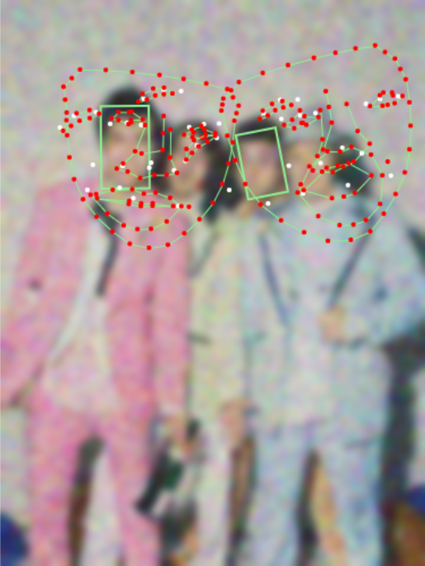
\includegraphics[scale=0.8]{faceNoise2115} \\ в) $\sigma^2=0.15$}
	\end{minipage}
	\caption{Распознавание лиц на изображениях после применения гауссовского фильтра с радиусом 21}
\end{figure}
Количество распознанных лиц на $\sigma^2=0.01$ уменьшилось до 3. На $\sigma^2=0.05$ количество лиц осталось прежним, но теперь удалось распознать крайнее лицо. Для изображения с $\sigma^2=0.15$ удалось добиться распознавания лиц до двух. Во всех случаях удалось лишь добиться распознавания лиц, определение местоположения рта, глаз и носа оказалось невозможным.
Исходя из этого можно сделать вывод, что при применении алгоритмов шумоподавления важно правильно оценивать параметры шума на изображении и уже на основании этого подбирать оптимальные параметры алгоритма.